\chapter{Dataset}
\label{chapter:dataset} 


\section{Introduction}

\lipsum[2-4]

\section{Clinical study design}

\lipsum[2-4]

\section{Instrumentation}

\lipsum[2-4]

\begin{figure}[tbh]
  \centering
  \subbottom[]{
    \label{fig:grasshopper:lens}
    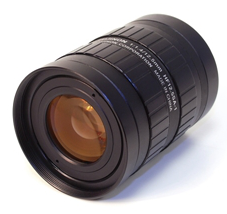
\includegraphics[width=0.2\linewidth,keepaspectratio=true]{fujinon-hf125sa_lens}
  } 
  \subbottom[]{
    \label{fig:grasshopper:camera}
    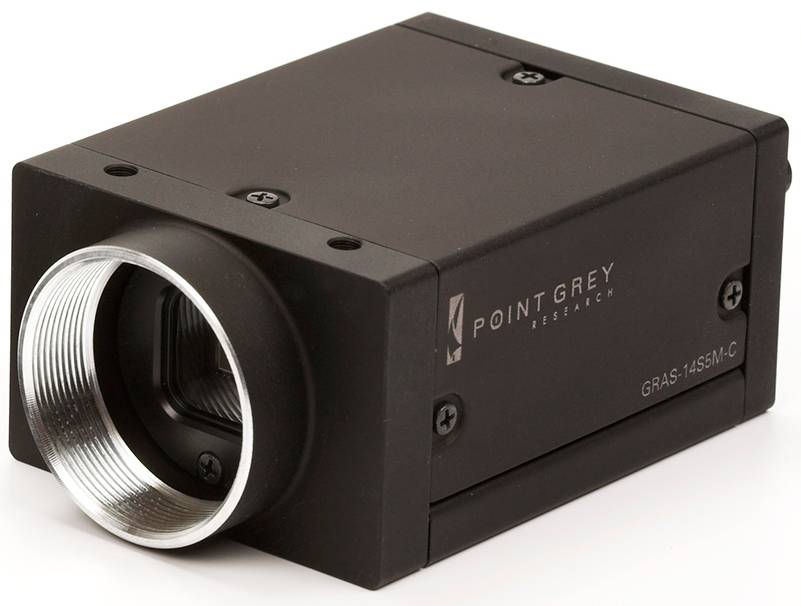
\includegraphics[width=0.22\linewidth,keepaspectratio=true]{grasshopper2}
  }
  \subbottom[]{
    \label{fig:grasshopper:sensor}
    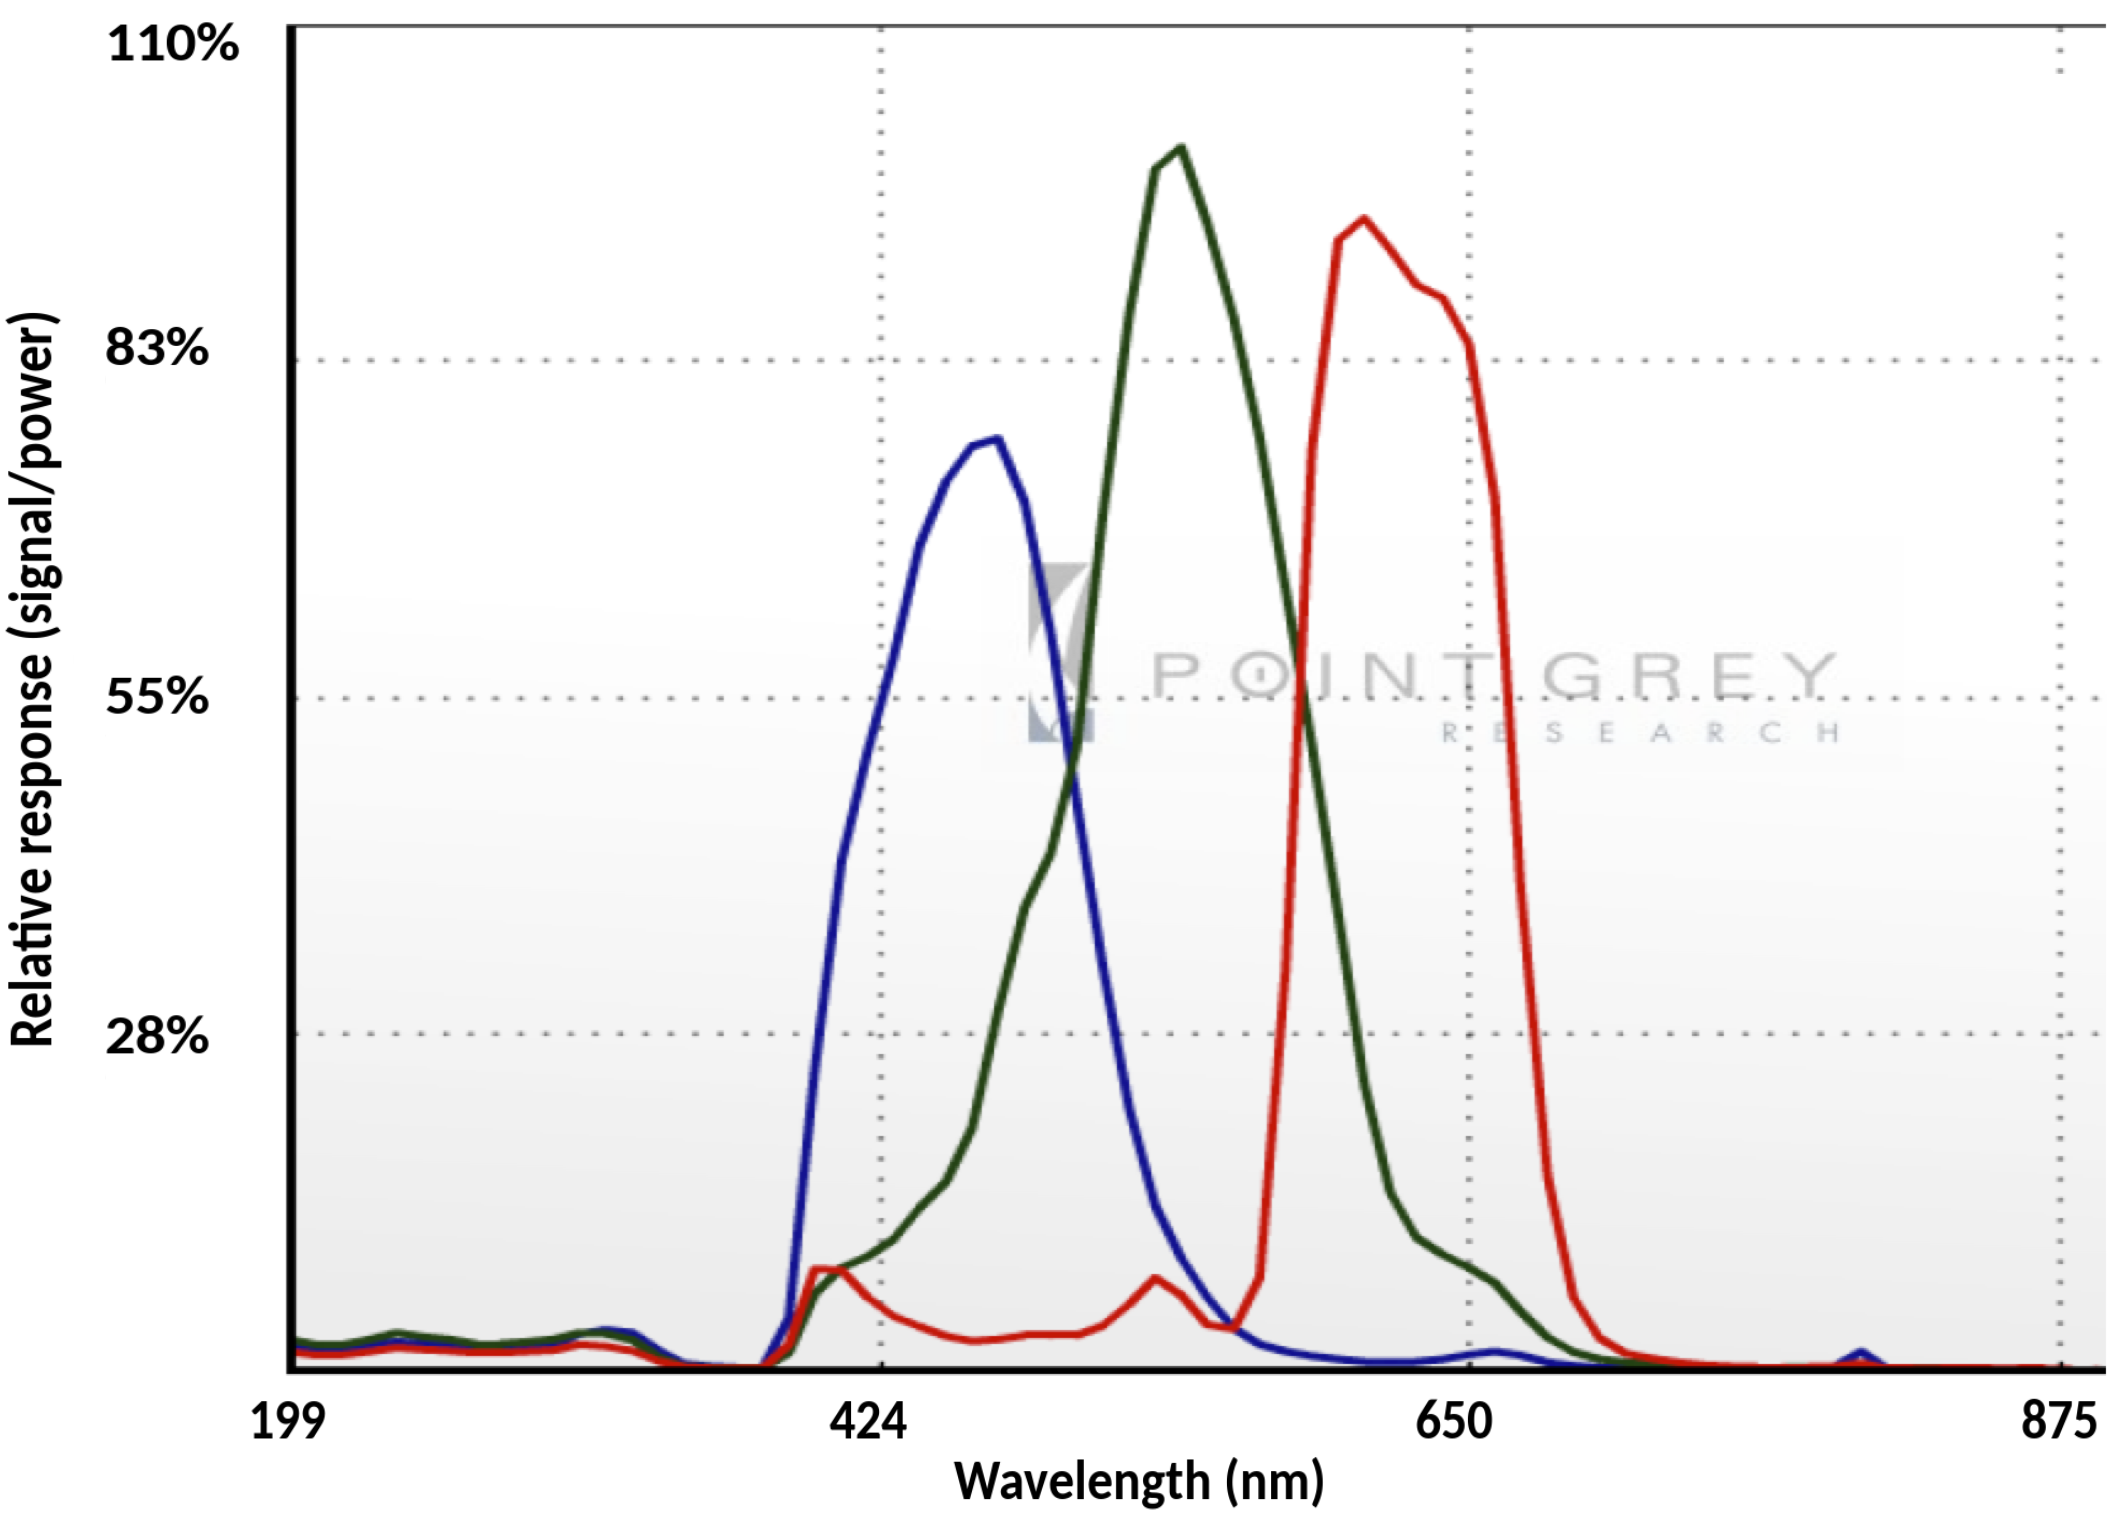
\includegraphics[width=0.45\linewidth,keepaspectratio=true]{grasshopper2_sensor}
  }
  \caption[The PointGrey Grasshopper2 video camera]
  {
  The video camera used in the study:
  \subcaptionref{fig:grasshopper:lens}   Fujinon HF12.5SA-1 lens,
  \subcaptionref{fig:grasshopper:camera} PointGrey Grasshopper2 camera module.
  \subcaptionref{fig:grasshopper:sensor} Response curve for the red, green and blue wavelengths from the image sensor inside the Grasshopper2 camera: Sony ICX625 2/3" progressive scan CCD (Source: PointGrey).
  }
  \label{fig:grasshopper}
\end{figure}

\Cref{fig:grasshopper} shows the video camera used in the study ...

\lipsum[2-4]

\Cref{table:grasshopper2_specs} describes the ...

\begin{table}[bth]
  \centering
  \caption[General features and specification for the PointGrey Grasshopper2 camera]
  {
  General features and specification for the PointGrey Grasshopper2 camera. (Source: PointGrey)}
  {\small
   \singleTableRowHeight
   \begin{tabular}{ll}
     \tableHeaderStart
        \tableHCell{Item} & \tableHCell{Description} \\
     \tableHeaderEnd
     Imaging Sensor        & Sony ICX625 2/3" progressive scan CCD \\
     Image size (pixels)   & 2448 (H) x 2048 (V)                   \\
     Pixel Size            & 3.45 \si{\micro\metre} x 3.45 \si{\micro\metre} \\
     A/D Converter         & AD9977 14-bit, dual-channel           \\
     Max frame rate        & 15 FPS                                \\
     Video Data Output     & 8, 12, 16 and 24-bit digital data     \\
     Gain \& Exposure                  & Automatic/Manual/One-Push              \\
     Lens Mount            & C-mount                                \\
     Interface             & Gigabit Ethernet                       \\
     Physical dimensions   & 44 (W) mm x 29 (H) mm x 58 (L) mm \\
     \hline 
   \end{tabular}
  }
  \label{table:grasshopper2_specs}
\end{table}

\lipsum[2-4]

\section{Patient population}

\lipsum[2-4]

\subsection{Demographics}

\lipsum[2-4]

\subsection{Vital signs}

\lipsum[2-4]

\section{Conclusion}

\lipsum[2-4]